\section{Experiments}
\subsection{Datasets and Metrics}
We conduct experiments on two datasets. One is a real world dataset.
In order to evaluate the strategy in a more comprehensive way, we
also perform experiments on a synthetic dataset. Details of the
processing of the datasets can be referred to the Appendix B.
\subsubsection{Yelp dataset}
The data is provided by Yelp Dataset Challenge, which mainly deals with review and business data to get user ratings for businesses and the city where business is located.
\subsubsection{Synthetic datasets}
We also generate a synthetic dataset to test the performance of the algorithms under different parameter settings. For this purpose, we generate 4 synthetic datasets with different situations of capacity conflicts when N is set to 5. Dataset 1 represents a situation where there is almost no capacity conflicts. Dataset 2 is a very balanced dataset. Dataset 3 represents a situation where the capacity conflicts are pretty prominent. Dataset 4 is a situation with serious conflicts. Each dataset contains 800 users and 50 services.
\subsubsection{Metrics}
 We measure the total quality of recommendations of each user and variance among Top-N Fairness of all users at the same time.
\subsection{Strategy Comparison}
In our experiments,  we compare our approach against the following two baseline methods.

\paragraph{Preempt Strategy} In this approach, each time a user comes, we check first N services in its original recommendation list one by one until a service with enough capacity is found. Then we allocate this service into the output recommendation list. This method is a kind of first-come first-served (FCFS) process scheduling algorithm which doesn't take the fairness into consideration.

\paragraph{Random Strategy} In this approach, each time a user comes, we check first N services in its original recommendation list one by one. For each service, we find all users in the dataset whose top-N original recommendation list contains this service. Then it will be randomly distributed to one of these users. This strategy can
also assure the Top-N Fairness in the long run.
\subsection{Results on Yelp Dataset}
We conduct 100 rounds of recommendations on a dynamic user set on the Yelp dataset, which contains the data of Phoenix and Toronto. In the experiment we set N to 5 and Arrival probability to 0.6, and Figure\ref{fig:Yelp} shows the results. 

\begin{figure}[h]
\centering
% 
\subfigure[Quality of Recommendation, Phoenix]{
\begin{minipage}[t]{0.2\linewidth}
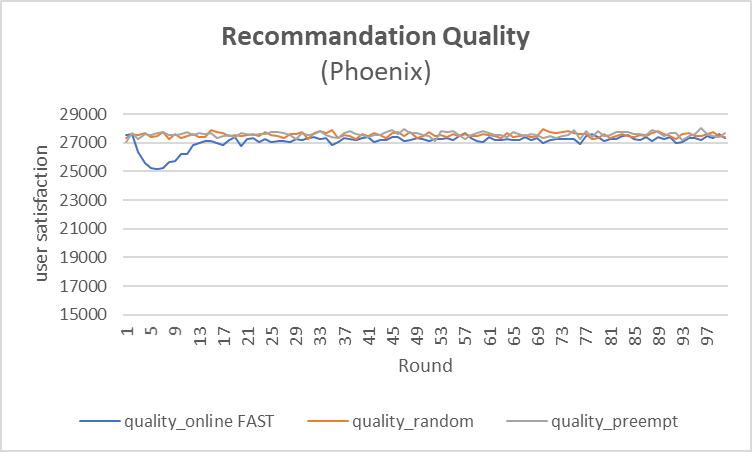
\includegraphics[width=3.7cm,height=2.5cm]{img/2_q_p.png}
%\caption{fig1}
\end{minipage}%
}%
\quad
\subfigure[Variance of Top-N Fairness,Phoenix]{
\begin{minipage}[t]{0.2\linewidth}
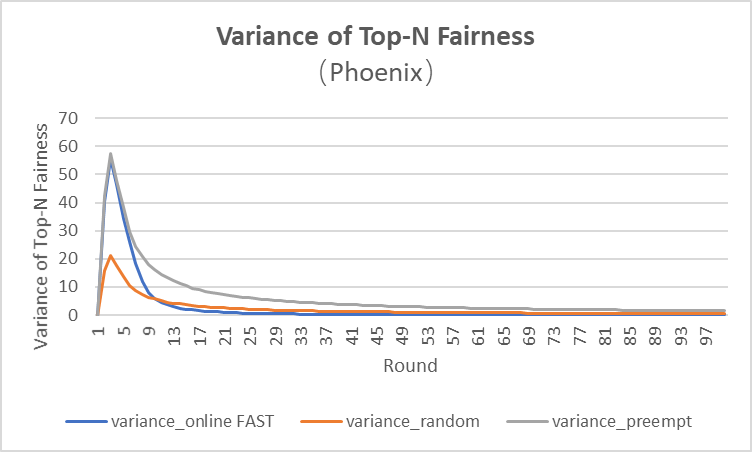
\includegraphics[width=3.7cm,height=2.5cm]{img/2_v_p.png}
%\caption{fig2}
\end{minipage}%
}%
\quad
\subfigure[Quality of Recommendation, Toronto ]{
\begin{minipage}[t]{0.2\linewidth}
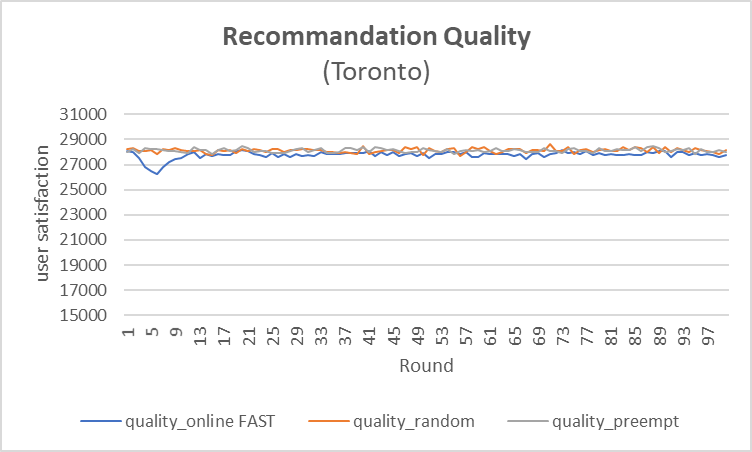
\includegraphics[width=3.7cm,height=2.5cm]{img/2_q_t.png}
%\caption{fig3}
\end{minipage}%
}%
\quad
\subfigure[Variance of Top-N Fairness, Toronto]{
\begin{minipage}[t]{0.2\linewidth}
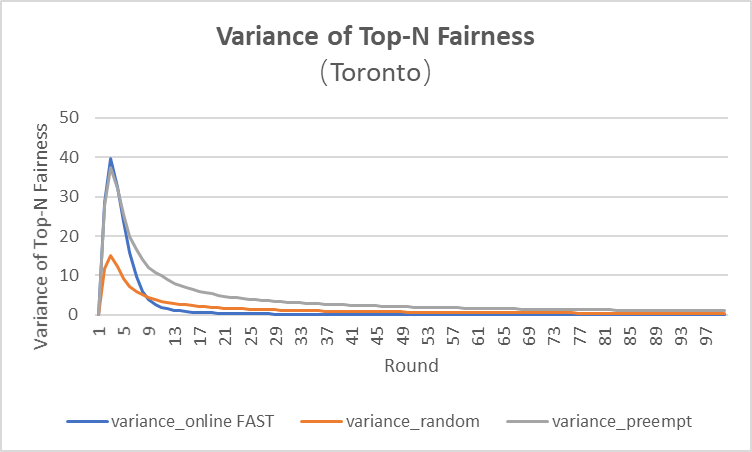
\includegraphics[width=3.7cm,height=2.5cm]{img/2_v_t.png}
%\caption{fig4}
\end{minipage}%
}%
\centering
\caption{Recommendation Quality under Different Levels of Capacity Constraints}
\label{fig:Yelp}
\end{figure}

It can be seen from Figure\ref{fig:Yelp} that our online-FAST's variance of Top-N Fairness approaches zero faster than other two strategy. What's more, its variance of fairness at the stable status is the least. When it comes to the quality of recommendations, we can see that these three strategies can reach the similar result.


\subsection{Results on Synthetic Dataset}
\paragraph{Comparisons between Different Levels of Capacity Constraints.} We conduct 100 rounds of recommendations on a dynamic user set on four synthetic datasets to compare the performance of algorithms in the cases of different levels of capacity conflicts. In four groups of experiments, N is uniformly set to 5 and probability of arrival is uniformly set to 0.6. Figure \ref{fig:RQ} and \ref{fig:V} show the results of quality and fairness of recommendations, respectively. It can be seen from Figure \ref{fig:RQ} that as capacity conflict being more intensive, quality of recommendations tends to decrease. The reason is when capacity conflict becomes more intensive, users have less chances to be assigned top-N services in his original list, which in turn leads to a decrease in quality. The less intensive the capacity conflict is, the better quality of recommendations our approach can achieve compared with the random strategy. Figure \ref{fig:V} shows that online-FAST arrives the stable status of fairness faster than preempt strategy and random strategy in all scenarios. What's more, its variance of fairness at the stable status is the least.
\begin{figure}[h]
\centering
% 
\subfigure[Synthetic Dataset 1]{
\begin{minipage}[t]{0.2\linewidth}
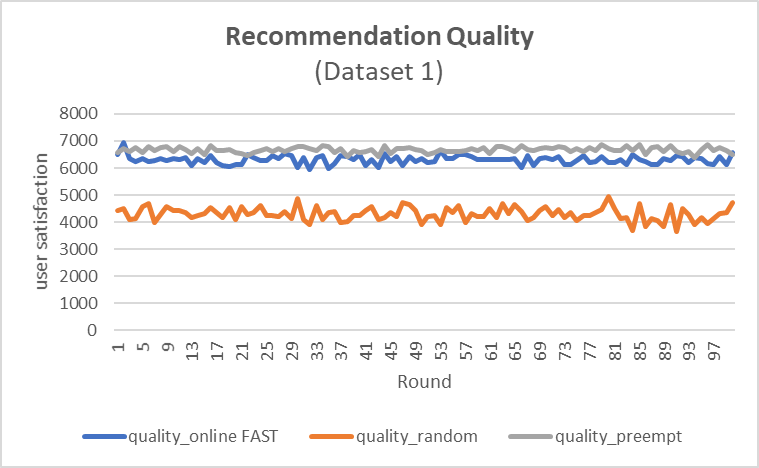
\includegraphics[width=3.7cm,height=2.5cm]{img/1_q_1.png}
%\caption{fig1}
\end{minipage}%
}%
\quad
\subfigure[Synthetic Dataset 2]{
\begin{minipage}[t]{0.2\linewidth}
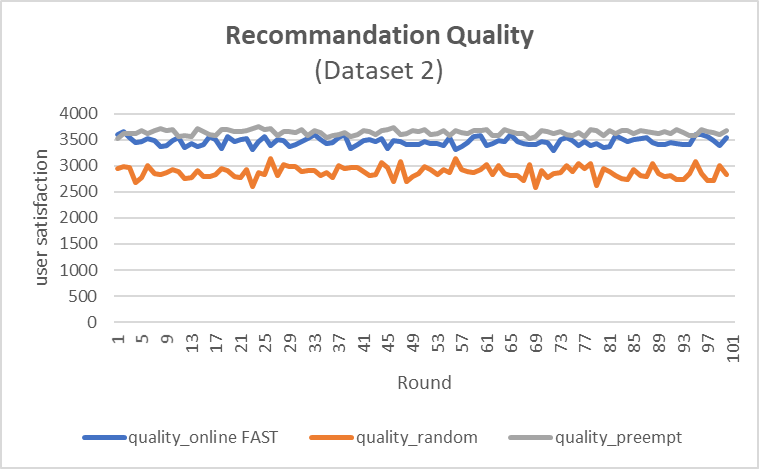
\includegraphics[width=3.7cm,height=2.5cm]{img/1_q_2.png}
%\caption{fig2}
\end{minipage}%
}%
\quad
\subfigure[Synthetic Dataset 3]{
\begin{minipage}[t]{0.2\linewidth}
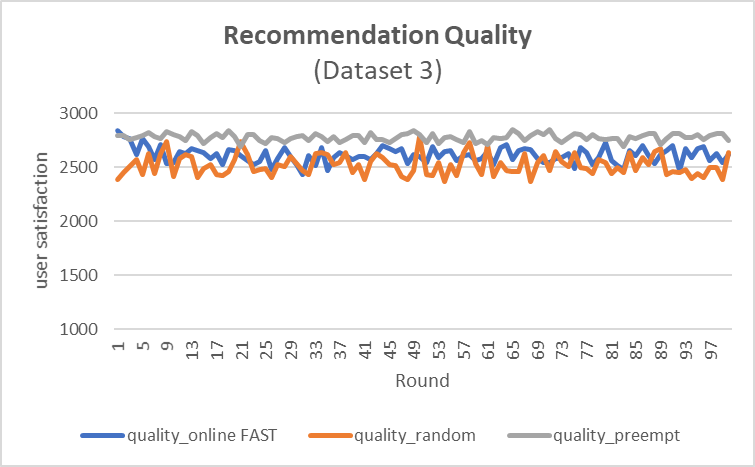
\includegraphics[width=3.7cm,height=2.5cm]{img/1_q_3.png}
%\caption{fig3}
\end{minipage}%
}%
\quad
\subfigure[Synthetic Dataset 4]{
\begin{minipage}[t]{0.2\linewidth}
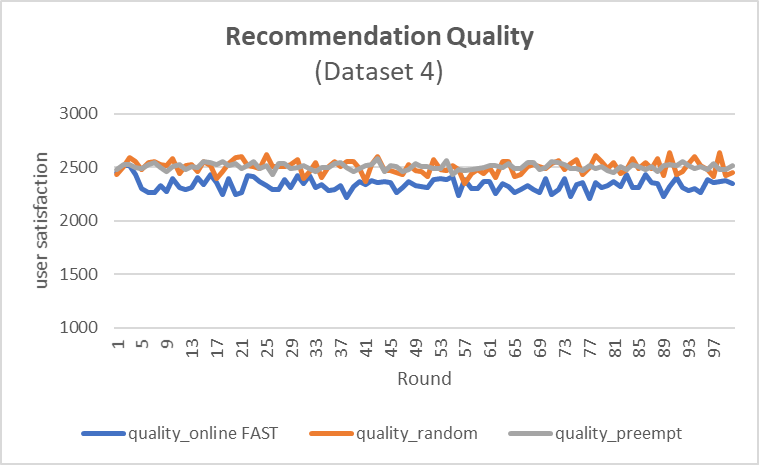
\includegraphics[width=3.7cm,height=2.5cm]{img/1_q_4.png}
%\caption{fig4}
\end{minipage}%
}%
\centering
\caption{Recommendation Quality under Different Levels of Capacity Constraints}
\label{fig:RQ}
\end{figure}

\begin{figure}[h]
\centering
\subfigure[Synthetic Dataset 1]{
\begin{minipage}[t]{0.2\linewidth}
\centering
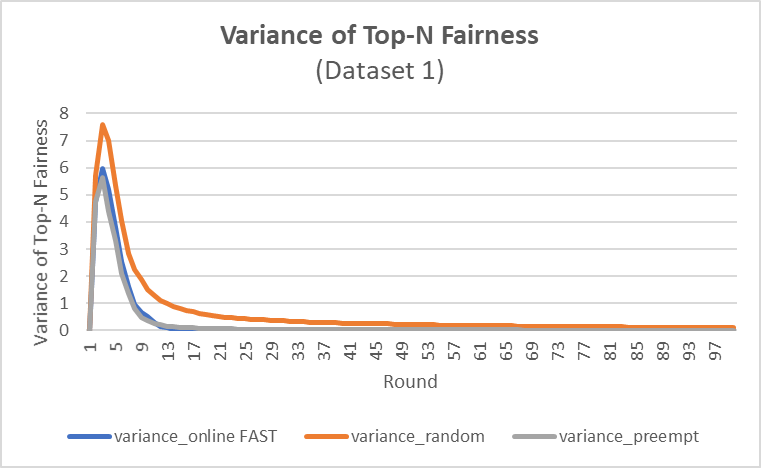
\includegraphics[width=3.7cm,height=2.5cm]{img/1_v_1.png}
%\caption{fig1}
\end{minipage}%
}%
\quad
\subfigure[Synthetic Dataset 2]{
\begin{minipage}[t]{0.2\linewidth}
\centering
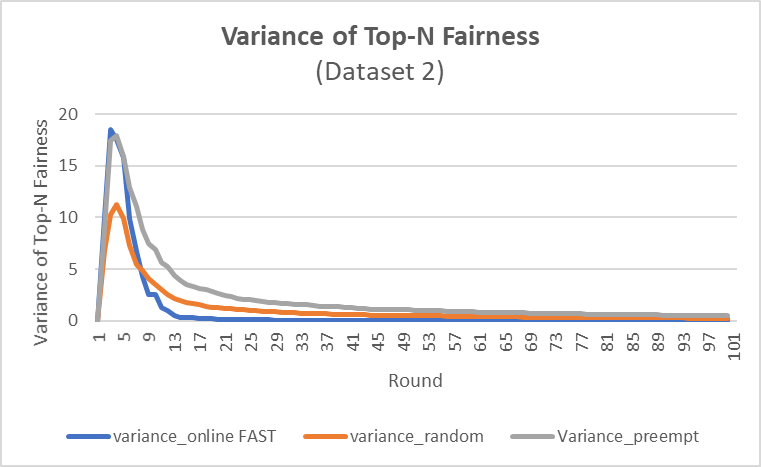
\includegraphics[width=3.7cm,height=2.5cm]{img/1_v_2.png}
%\caption{fig2}
\end{minipage}%
}%
\quad
\subfigure[Synthetic Dataset 3]{
\begin{minipage}[t]{0.2\linewidth}
\centering
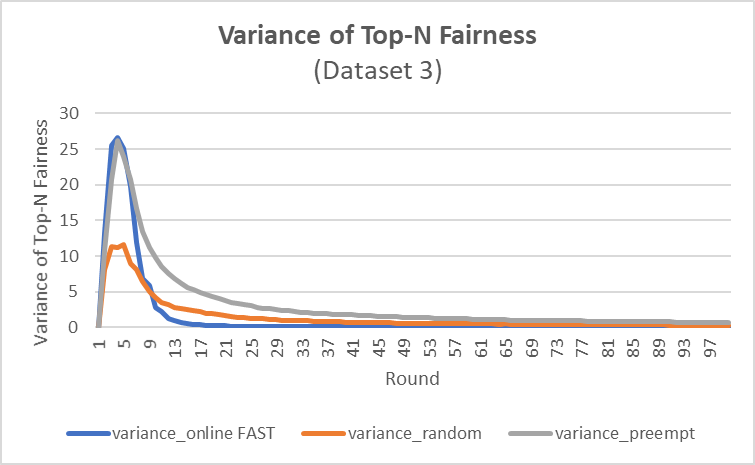
\includegraphics[width=3.7cm,height=2.5cm]{img/1_v_3.png}
%\caption{fig3}
\end{minipage}%
}%
\quad
\subfigure[Synthetic Dataset 4]{
\begin{minipage}[t]{0.2\linewidth}
\centering
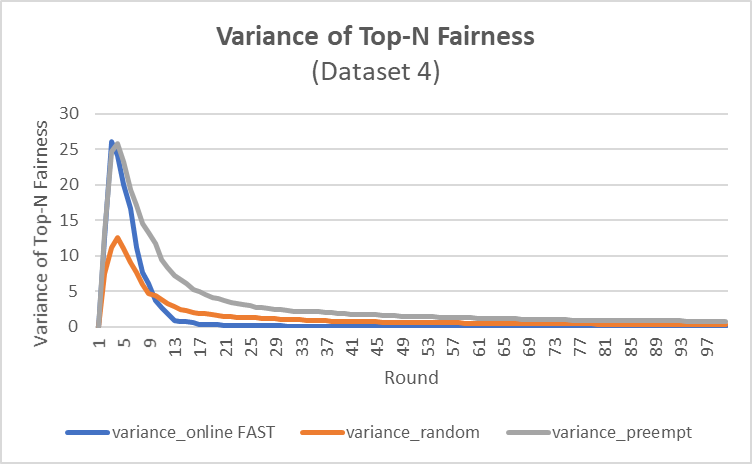
\includegraphics[width=3.7cm,height=2.5cm]{img/1_v_4.png}
%\caption{fig4}
\end{minipage}%
}%
\centering
\caption{Variance of Top-N Fairness under Different Levels of Capacity Constraints}
\label{fig:V}
\end{figure}

\paragraph{Comparisons between Different Probability of Arrival.}  Figure \ref{fig:RQ-A} and \ref{fig:V-A} show the performance of algorithms under different arrival probability. This experiment is performed on Synthetic Dataset 2 on a dynamic user set, and a total of 100 rounds of recommendations are carried out for each experiment.
As can be seen from the figure\ref{fig:RQ-A}, as the arrival probability rises, overall recommendation quality improves, but the rate of growth in our online-FAST is less than that of the random strategy. So the smaller the arrival probability is, the more advantage online-FAST have over them with respect to recommendation quality. Figure \ref{fig:V-A} shows that online-FAST arrives the stable status of fairness faster than preempt strategy and random strategy in all scenarios. What's more, its variance of fairness at the stable status is the least.
\begin{figure}[h]
\centering
\subfigure[Arrive Probability=0.5]{
\begin{minipage}[t]{0.2\linewidth}
\centering
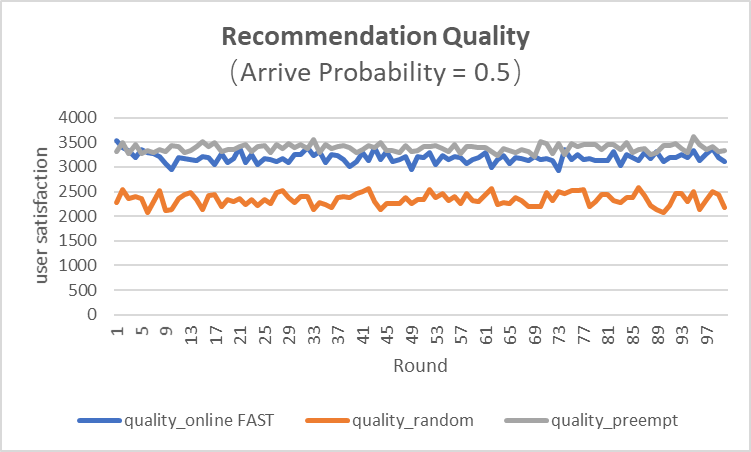
\includegraphics[width=3.7cm,height=2.5cm]{img/3_q_0.5.png}
%\caption{fig1}
\end{minipage}%
}%
\quad
\subfigure[Arrive Probability=0.6]{
\begin{minipage}[t]{0.2\linewidth}
\centering
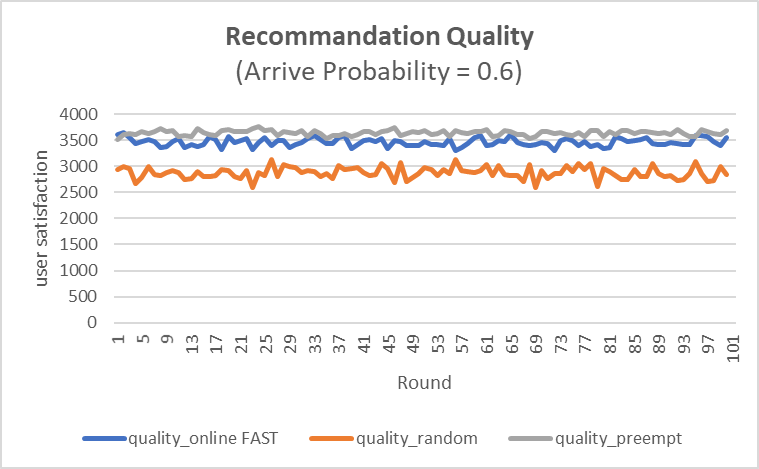
\includegraphics[width=3.7cm,height=2.5cm]{img/3_q_0.6.png}
%\caption{fig2}
\end{minipage}%
}%
\quad
\subfigure[Arrive Probability=0.7]{
\begin{minipage}[t]{0.2\linewidth}
\centering
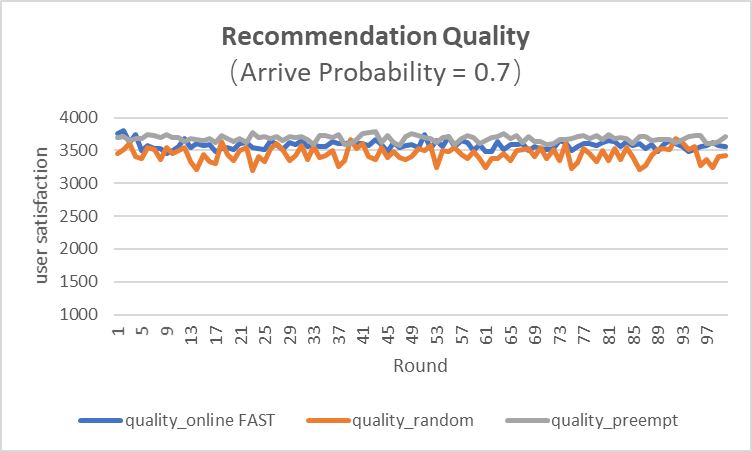
\includegraphics[width=3.7cm,height=2.5cm]{img/3_q_0.7.png}
%\caption{fig3}
\end{minipage}%
}%
\quad
\subfigure[Arrive Probability=0.8]{
\begin{minipage}[t]{0.2\linewidth}
\centering
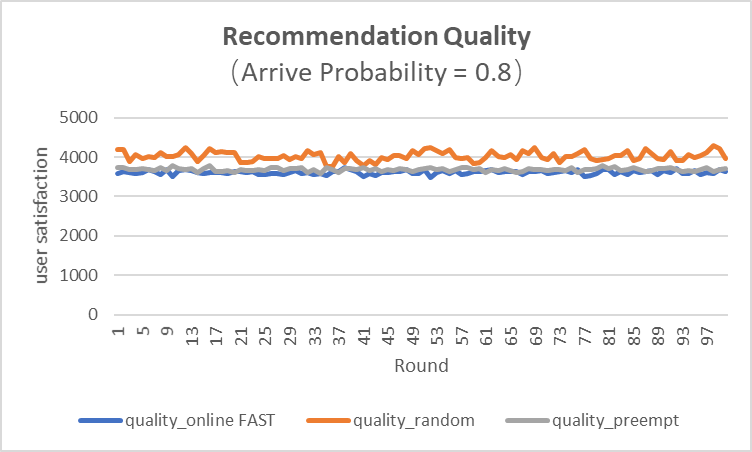
\includegraphics[width=3.7cm,height=2.5cm]{img/3_q_0.8.png}
%\caption{fig4}
\end{minipage}%
}%
\centering
\caption{Recommendation Quality with Different Arriving Probability}
\label{fig:RQ-A}
\end{figure}




\begin{figure}[h]
\centering
\subfigure[Arrive Probability=0.5]{
\begin{minipage}[t]{0.2\linewidth}
\centering
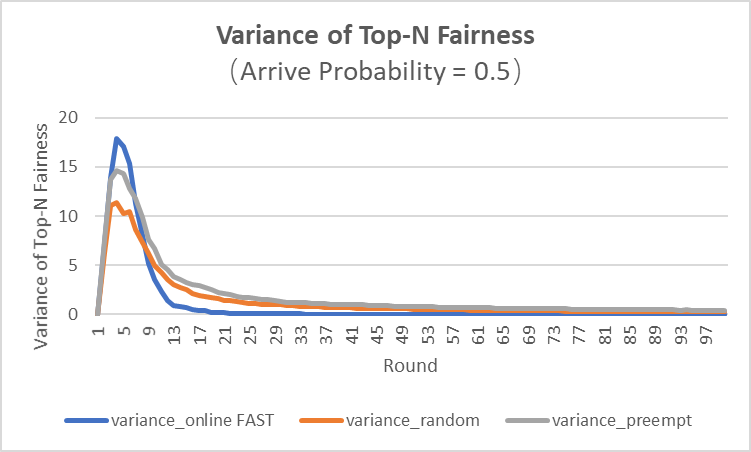
\includegraphics[width=3.7cm,height=2.5cm]{img/3_v_0.5.png}
%\caption{fig1}
\end{minipage}%
}%
\quad
\subfigure[Arrive Probability=0.6]{
\begin{minipage}[t]{0.2\linewidth}
\centering
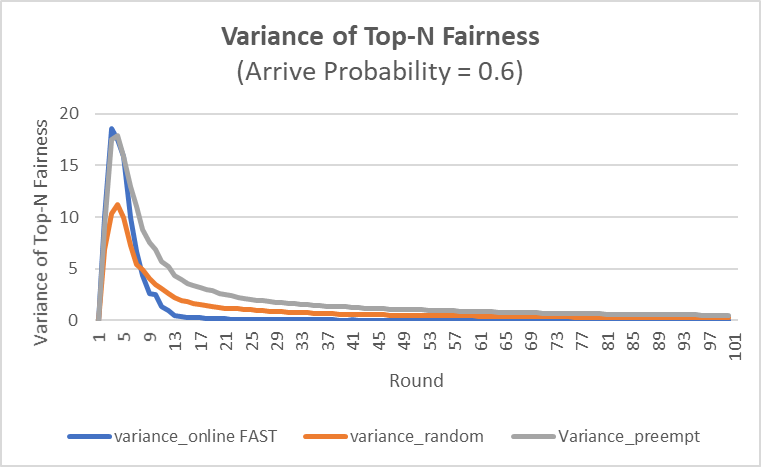
\includegraphics[width=3.7cm,height=2.5cm]{img/3_v_0.6.png}
%\caption{fig2}
\end{minipage}%
}%
\quad
\subfigure[Arrive Probability=0.7]{
\begin{minipage}[t]{0.2\linewidth}
\centering
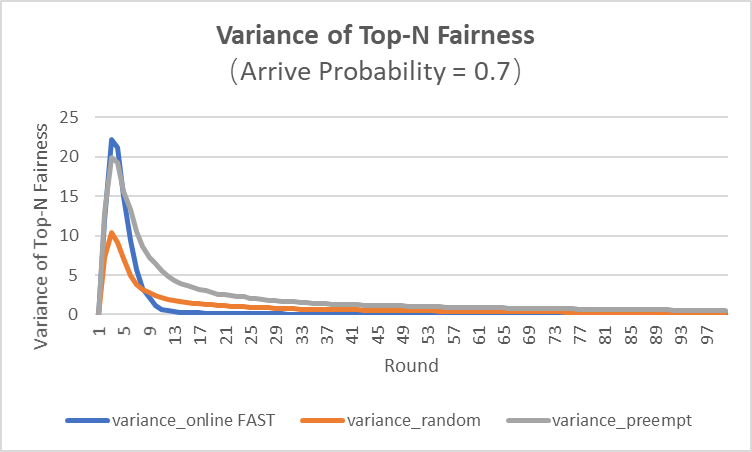
\includegraphics[width=3.7cm,height=2.5cm]{img/3_v_0.7.png}
%\caption{fig3}
\end{minipage}%
}%
\quad
\subfigure[Arrive Probability=0.8]{
\begin{minipage}[t]{0.2\linewidth}
\centering
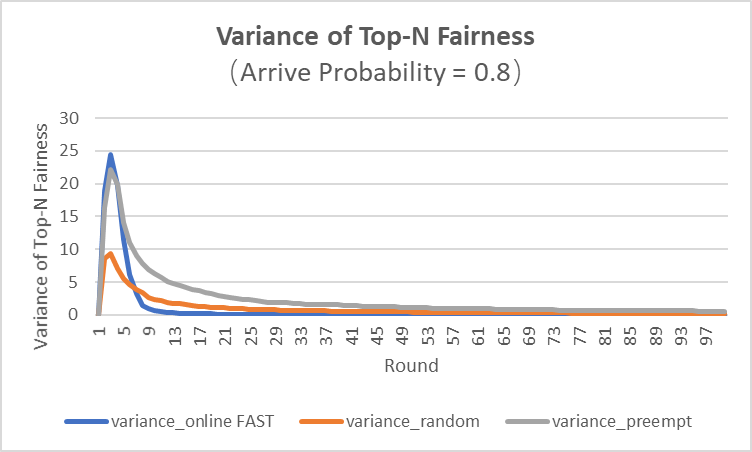
\includegraphics[width=3.7cm,height=2.5cm]{img/3_v_0.8.png}
%\caption{fig4}
\end{minipage}%
}%
\centering
\caption{Variance of Fairness with Different Arrive Probability}
\label{fig:V-A}
\end{figure}

\paragraph{Comparisons between Different N.}  Figure \ref{fig:RQ-N} and \ref{fig:V-N} show the performance of algorithms under different N. This experiment is performed on Synthetic Dataset 2 on a dynamic user set, and a total of 100 rounds of recommendations are carried out for each experiment. As can be seen from the figure\ref{fig:RQ-N}, as N rises, overall recommendation quality improves at first, but when N becomes large enough, it starts to decrease. The reason is the impacts of the services in
the lower positions in the original recommendation list are smaller.

 Figure \ref{fig:V-N} shows that online-FAST arrives the stable status of fairness faster than preempt strategy and random strategy in all scenarios. What's more, its variance of fairness at the stable status is the least. As N rises, the variance of Top-N Fairness rises instead. This shows that a longer top-N recommendation list will
not bring benefits to the recommendation quality but impair the
fairness.

\begin{figure}[h]
\centering
\subfigure[Top-N = 3]{
\begin{minipage}[t]{0.16\linewidth}
\centering
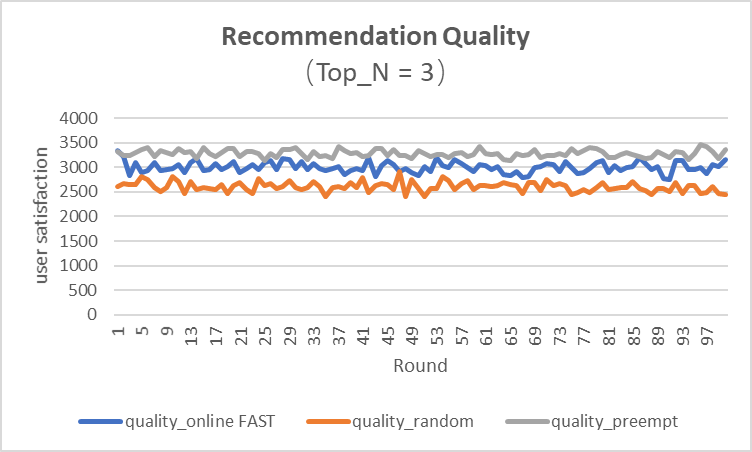
\includegraphics[width=3cm,height=2.2cm]{img/4_q_3.png}
%\caption{fig1}
\end{minipage}%
}%
\quad
\subfigure[Top-N = 5]{
\begin{minipage}[t]{0.16\linewidth}
\centering
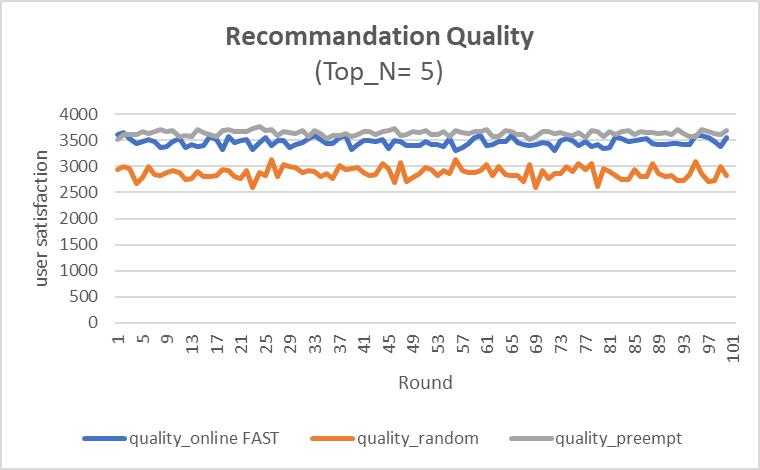
\includegraphics[width=3cm,height=2.2cm]{img/4_q_5.png}
%\caption{fig2}
\end{minipage}%
}%
\quad
\subfigure[Top-N = 7]{
\begin{minipage}[t]{0.16\linewidth}
\centering
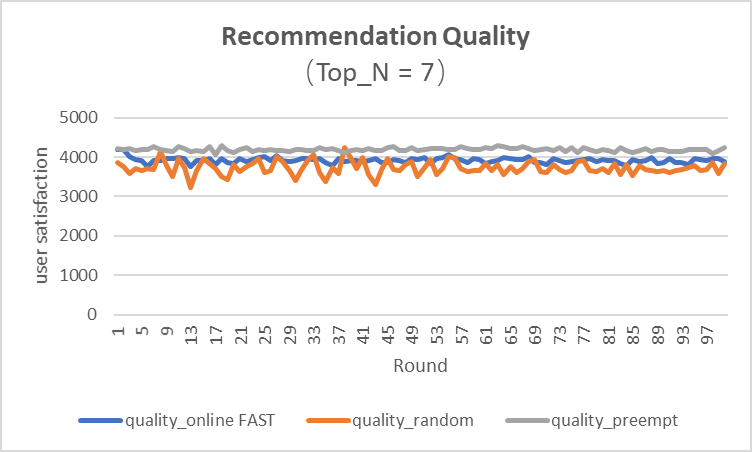
\includegraphics[width=3cm,height=2.2cm]{img/4_q_7.png}
%\caption{fig3}
\end{minipage}%
}%
\quad
\subfigure[Top-N = 10]{
\begin{minipage}[t]{0.16\linewidth}
\centering
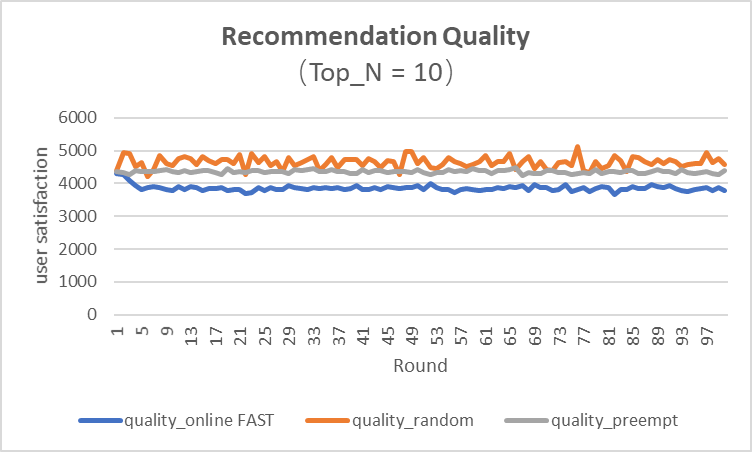
\includegraphics[width=3cm,height=2.2cm]{img/4_q_10.png}
%\caption{fig4}
\end{minipage}%
}%
\quad
\subfigure[Top-N = 15]{
\begin{minipage}[t]{0.16\linewidth}
\centering
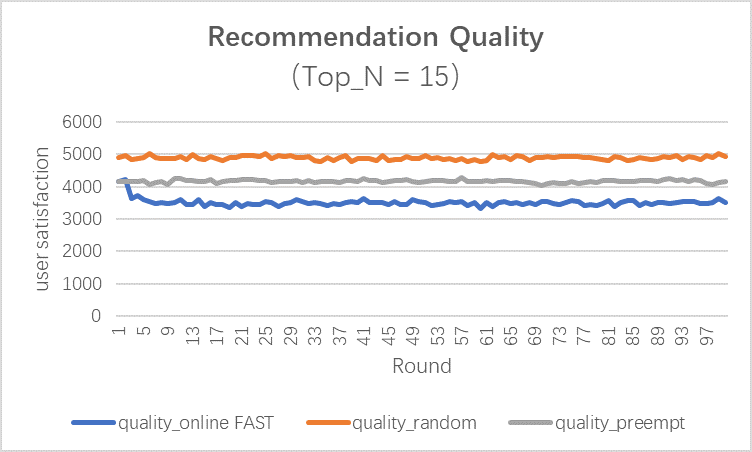
\includegraphics[width=3cm,height=2.2cm]{img/4_q_15.png}
%\caption{fig5}
\end{minipage}%
}%
\centering
\caption{Recommendation Quality under Different N}
\label{fig:RQ-N}
\end{figure}



\begin{figure}[h]
\centering
\subfigure[Top-N = 3]{
\begin{minipage}[t]{0.16\linewidth}
\centering
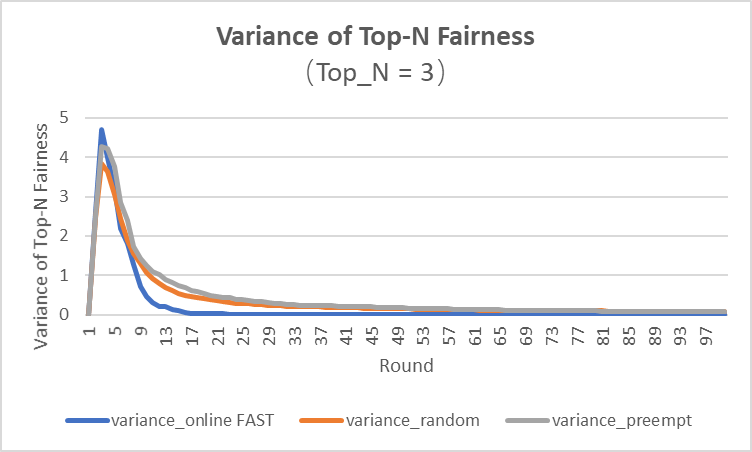
\includegraphics[width=3cm,height=2.2cm]{img/4_v_3.png}
%\caption{fig1}
\end{minipage}%
}%
\quad
\subfigure[Top-N = 5]{
\begin{minipage}[t]{0.16\linewidth}
\centering
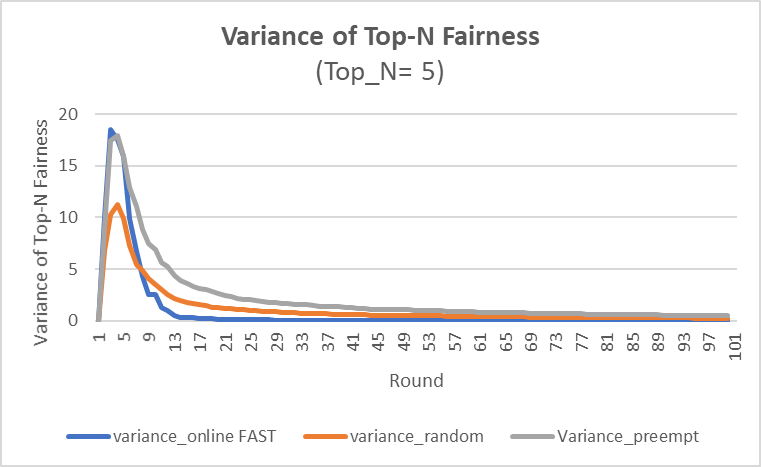
\includegraphics[width=3cm,height=2.2cm]{img/4_v_5.png}
%\caption{fig2}
\end{minipage}%
}%
\quad
\subfigure[Top-N = 7]{
\begin{minipage}[t]{0.16\linewidth}
\centering
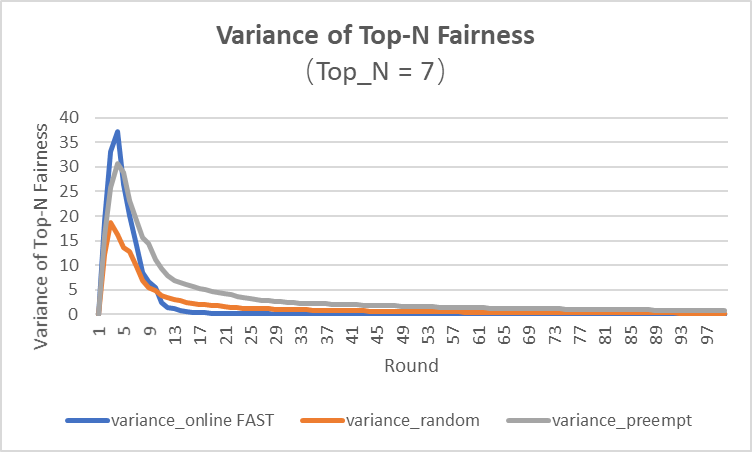
\includegraphics[width=3cm,height=2.2cm]{img/4_v_7.png}
%\caption{fig3}
\end{minipage}%
}%
\quad
\subfigure[Top-N = 10]{
\begin{minipage}[t]{0.16\linewidth}
\centering
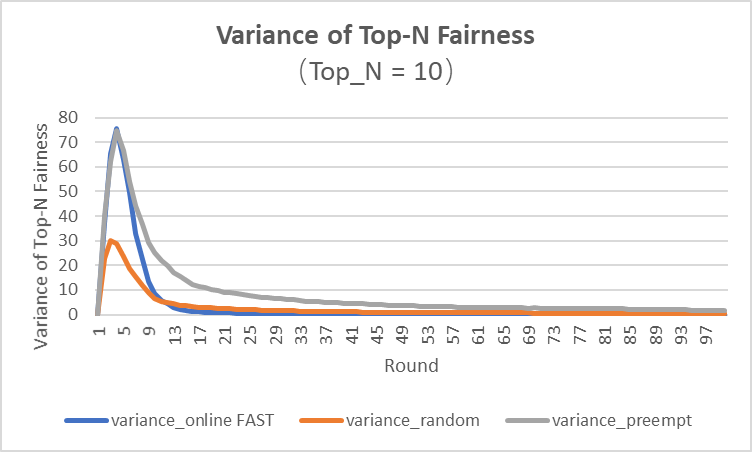
\includegraphics[width=3cm,height=2.2cm]{img/4_v_10.png}
%\caption{fig4}
\end{minipage}%
}%
\quad
\subfigure[Top-N = 15]{
\begin{minipage}[t]{0.16\linewidth}
\centering
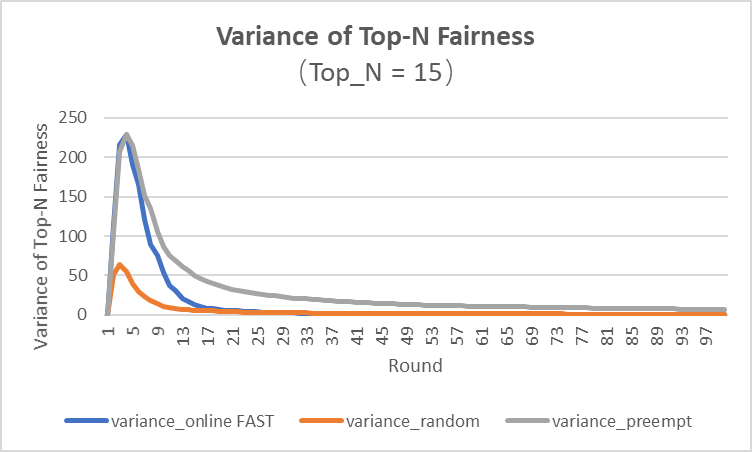
\includegraphics[width=3cm,height=2.2cm]{img/4_v_15.png}
%\caption{fig5}
\end{minipage}%
}%
\centering
\caption{Variance of Top-N Fairness under Different N}
\label{fig:V-N}
\end{figure}